\documentclass[20pt, a1paper, portrait]{tikzposter}

% --- Core Packages ---
\usepackage[utf8]{inputenc}
\usepackage{amsmath,amssymb,amsfonts}
\usepackage{booktabs}
\usepackage{tabularx}
\usepackage{colortbl}
\usepackage{graphicx}
\usepackage{siunitx}
\usepackage{tikz}
\usetikzlibrary{shapes.geometric, arrows.meta, positioning, fit}

\tikzposterlatexaffectionproofoff

% --- Official University of Moratuwa Academic Color Palette ---
\definecolor{MoratuwaNavy}{HTML}{002147}
\definecolor{MoratuwaBlue}{HTML}{0B3C5D}
\definecolor{MoratuwaAccent}{HTML}{1976D2}
\definecolor{MoratuwaGold}{HTML}{D9A74A}
\definecolor{MoratuwaLightGold}{HTML}{FFF4DC}
\definecolor{PosterBg}{HTML}{F6F8FA}
\definecolor{CardWhite}{HTML}{FFFFFF}
\definecolor{TextDark}{HTML}{1A202C}
\definecolor{TableHeadBg}{HTML}{E2E8F0}
\definecolor{HighlightRow}{HTML}{E8F4FD}

% --- Tikzposter Theme Customization ---
\usetheme{Default}
\colorlet{backgroundcolor}{PosterBg}
\colorlet{framecolor}{MoratuwaBlue}
\colorlet{titlefgcolor}{white}
\colorlet{titlebgcolor}{MoratuwaNavy}
\colorlet{blocktitlebgcolor}{MoratuwaNavy}
\colorlet{blocktitlefgcolor}{white}
\colorlet{blockbodybgcolor}{CardWhite}
\colorlet{blockbodyfgcolor}{TextDark}

% --- Metadata ---
\title{Automated Sim-to-Real Deployment Framework for\\Reinforcement Learning on Resource-Constrained MCUs}

\author{\textbf{Nidharshan V.}$^{1}$, \textbf{Yasantha Niroshana}$^{2}$, \textbf{Odil Janandith}$^{2}$, \textbf{Sulochana Sooriyaarachchi}$^{1}$}

\institute{%
$^{1}$Department of Computer Science \& Engineering, University of Moratuwa, Sri Lanka \quad
$^{2}$RoboticGen (Pvt) Ltd, Sri Lanka\\
\textbf{\color{MoratuwaGold}ERU Research Symposium 2026} --- Engineering Research Unit, Faculty of Engineering
}

% --- Custom Header Banner ---
\makeatletter
\definetitlestyle{MoratuwaBanner}{
    width=\paperwidth, roundedcorners=0, linewidth=0pt, innersep=1.2cm,
    titletotopverticalspace=0mm, titletoblockverticalspace=18mm,
    titlegraphictotitledistance=0pt
}{
   \draw[draw=none, fill=MoratuwaNavy]%
   (\titleposleft,\titleposbottom) rectangle (\titleposright,\titlepostop); %
   \draw[draw=none, fill=MoratuwaGold]%
   (\titleposleft,\titleposbottom) rectangle (\titleposright,\titleposbottom+0.35cm); %
}
\usetitlestyle{MoratuwaBanner}

\gdef\TP@maketitle{
  \vspace{-0.2cm}
  \begin{minipage}[c]{0.73\linewidth}
    \raggedright
    \color{white}
    {\bfseries\fontsize{34}{40}\selectfont \@title \par}
    \vspace{0.4cm}
    {\color{MoratuwaLightGold}\fontsize{21}{26}\selectfont \@author \par}
    \vspace{0.25cm}
    {\color{white!90}\fontsize{15}{20}\selectfont \@institute \par}
  \end{minipage}%
  \hfill
  \begin{minipage}[c]{0.25\linewidth}
    \raggedleft
    \setlength{\fboxrule}{2.5pt}%
    \setlength{\fboxsep}{10pt}%
    \fcolorbox{MoratuwaGold}{white}{\includegraphics[height=3.2cm,keepaspectratio]{paper/eru_logo.png}}
  \end{minipage}
}
\makeatother

\begin{document}
\maketitle

\begin{columns}

% ==============================================================================
% LEFT COLUMN
% ==============================================================================
\column{0.5}

% --- Block 1: Problem Scenario & Motivation ---
\block{\bfseries 1. Problem Scenario \& Motivation}{
  \normalsize
  \textbf{The Scenario:} While reinforcement learning (RL) policies achieve dynamic agility in high-fidelity physics simulations, transferring them to ultra-low-cost, resource-constrained microcontrollers ($<$520\,kB RAM, bare-metal) requires tedious manual weight translation, custom forward passes, and error-prone peripheral driver programming.

  \vspace{0.3em}
  \textbf{Key Objectives \& Proposed Framework:}
  \begin{itemize}
    \setlength{\itemsep}{0.18em}
    \item \textbf{Dual-Target Export:} Compile PyTorch / Stable-Baselines3 actors directly into zero-allocation C headers or precompiled MicroPython bytecode (\texttt{.mpy}).
    \item \textbf{Declarative Loop Synthesis:} Generate complete 50\,Hz control firmware (\texttt{main.py} / C loop) from a single \texttt{config.yaml} specifying I2C IMU pins, normalization scales, and safety delta clipping.
    \item \textbf{Guaranteed Determinism:} Dual static stack buffers eliminate runtime heap allocations (\texttt{malloc}), preventing memory fragmentation and latency spikes.
  \end{itemize}
}

% --- Block 2: System Architecture ---
\block{\bfseries 2. System Architecture \& Pipeline}{
  \centering
  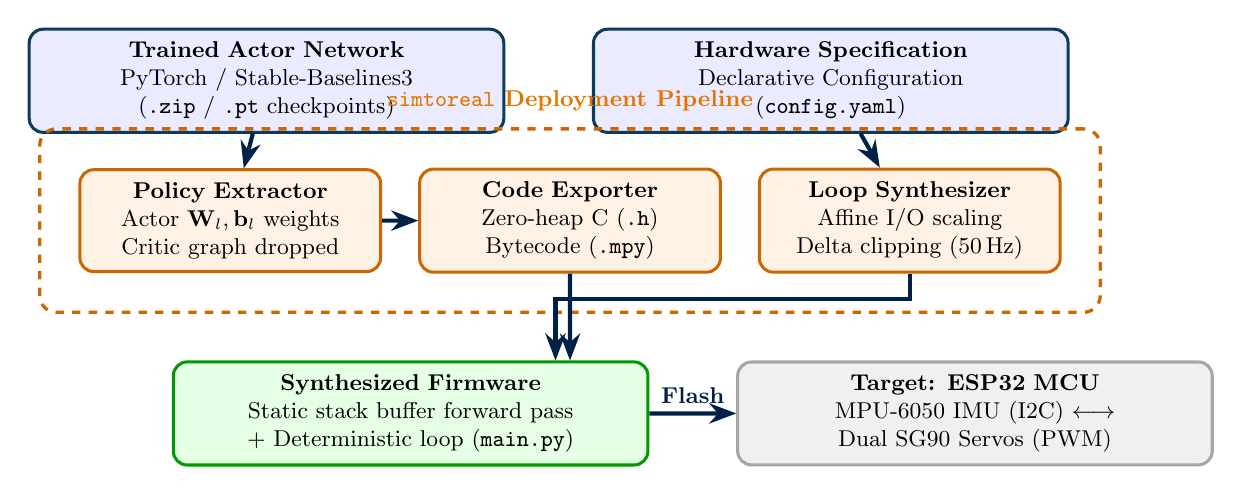
\begin{tikzpicture}[
      scale=0.92, every node/.style={transform shape},
      box/.style={draw, rounded corners=5pt, font=\small, align=center, inner sep=5pt, line width=1.1pt},
      inbox/.style={box, fill=blue!8, draw=MoratuwaBlue},
      core/.style={box, fill=orange!10, draw=orange!80!black},
      artbox/.style={box, fill=green!10, draw=green!60!black},
      mcu/.style={box, fill=gray!12, draw=gray!70},
      arrow/.style={-{Stealth[scale=1.0]}, draw=MoratuwaNavy, line width=1.5pt}
  ]
      % Inputs
      \node[inbox, text width=6.2cm] (m) {\textbf{Trained Actor Network}\\PyTorch / Stable-Baselines3\\(\texttt{.zip} / \texttt{.pt} checkpoints)};
      \node[inbox, text width=6.2cm, right=1.2cm of m] (c) {\textbf{Hardware Specification}\\Declarative Configuration\\(\texttt{config.yaml})};

      % Coordinates & Core Framework Nodes
      \coordinate[below=1.2cm of m, xshift=-0.5cm] (ext_pos);
      \node[core, text width=3.8cm] (ext) at (ext_pos) {\textbf{Policy Extractor}\\Actor $\mathbf{W}_l, \mathbf{b}_l$ weights\\Critic graph dropped};
      \node[core, text width=3.8cm, right=0.5cm of ext] (exp) {\textbf{Code Exporter}\\Zero-heap C (\texttt{.h})\\Bytecode (\texttt{.mpy})};
      \node[core, text width=3.8cm, right=0.5cm of exp] (syn) {\textbf{Loop Synthesizer}\\Affine I/O scaling\\Delta clipping (50\,Hz)};

      % Container Box around core framework
      \node[draw=orange!80!black, fill=none, rounded corners=6pt, dashed, line width=1.2pt,
            fit=(ext) (exp) (syn), inner sep=14pt,
            label={[font=\small\bfseries, text=orange!90!black, yshift=3pt]above:\texttt{simtoreal} Deployment Pipeline}] (box_lib) {};

      % Generated Firmware & Target
      \node[artbox, text width=6.2cm, below=1.2cm of exp, xshift=-2.2cm] (out) {\textbf{Synthesized Firmware}\\Static stack buffer forward pass\\+ Deterministic loop (\texttt{main.py})};
      \node[mcu, text width=6.2cm, right=1.2cm of out] (hw) {\textbf{Target: ESP32 MCU}\\MPU-6050 IMU (I2C) $\longleftrightarrow$\\Dual SG90 Servos (PWM)};

      % Connectors
      \draw[arrow] (m) -- (ext);
      \draw[arrow] (ext) -- (exp);
      \draw[arrow] (c) -- (syn);
      \draw[arrow] (exp) -- (out.north -| exp);
      \draw[arrow] (syn.south) -- ++(0,-0.35) -| ([xshift=2.0cm]out.north);
      \draw[arrow] (out) -- node[above, font=\small\bfseries, text=MoratuwaNavy] {Flash} (hw);
  \end{tikzpicture}
  \vspace{0.2em}
  
  \raggedright
  \small
  \textbf{Pipeline Flow:} (1) Extract weights $\rightarrow$ (2) Export zero-heap C / bytecode $\rightarrow$ (3) Synthesize 50\,Hz I2C/PWM control loop.
}

% --- Block 3: Literature Review Table ---
\block{\bfseries 3. Literature Review \& Framework Comparison}{
  \small
  \setlength{\tabcolsep}{4.5pt}
  \renewcommand{\arraystretch}{1.18}
  \begin{tabularx}{\linewidth}{p{4.0cm}p{4.2cm}p{2.6cm}p{4.0cm}X}
    \toprule
    \rowcolor{TableHeadBg}
    \textbf{Framework} & \textbf{Target Hardware} & \textbf{RAM Usage} & \textbf{Python RL Stack} & \textbf{Key Limitation / Feature} \\
    \midrule
    \textbf{ROS 2 / Orbit} & Linux SBCs / x86 \newline(RPi 4, Jetson) & $>$100\,MB & Native SB3 / Torch & High OS overhead; cannot run bare-metal microcontrollers. \\
    \textbf{TFLM} & Edge MCUs \newline(Cortex-M, ESP32) & 20--50\,kB & TensorFlow only \newline(No direct SB3) & General tensor interpreter runtime adds overhead for compact MLPs. \\
    \textbf{MCUNet} & Microcontrollers \newline(Cortex-M7) & 30--100\,kB & PyTorch Vision & Tailored for visual CNNs; no continuous RL control loops. \\
    \textbf{RLtools} & Microcontrollers \newline\& Bare-metal & $<$10\,kB & Custom C++ only \newline(No PyTorch/SB3) & Requires training inside proprietary C++ framework; no standard PyTorch. \\
    \rowcolor{HighlightRow}
    \textbf{\texttt{simtoreal}} \newline\textbf{(Ours)} & \textbf{Bare-Metal MCUs} \newline\textbf{(ESP32, RP2040)} & \textbf{$<$19\,kB Flash} \newline\textbf{0 Heap (C)} & \textbf{Direct SB3 \&} \newline\textbf{PyTorch Import} & \textbf{Automated peripheral drivers, zero-heap C headers, declarative YAML.} \\
    \bottomrule
  \end{tabularx}
}

% ==============================================================================
% RIGHT COLUMN
% ==============================================================================
\column{0.5}

% --- Block 4: Experimental Testbed: Robo1 ---
\block{\bfseries 4. Experimental Testbed: \textit{Robo1}}{
  \centering
  \begin{minipage}{0.44\linewidth}
    \centering
    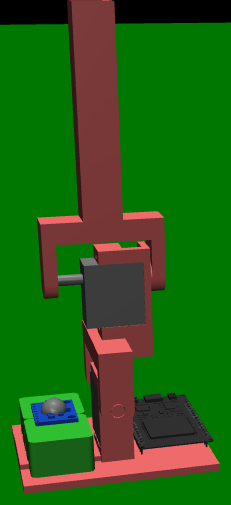
\includegraphics[height=7.4cm, keepaspectratio]{robo_sim.png}\\[0.2em]
    \small \textbf{(a) MuJoCo Simulation Model}
  \end{minipage}
  \hfill
  \begin{minipage}{0.53\linewidth}
    \centering
    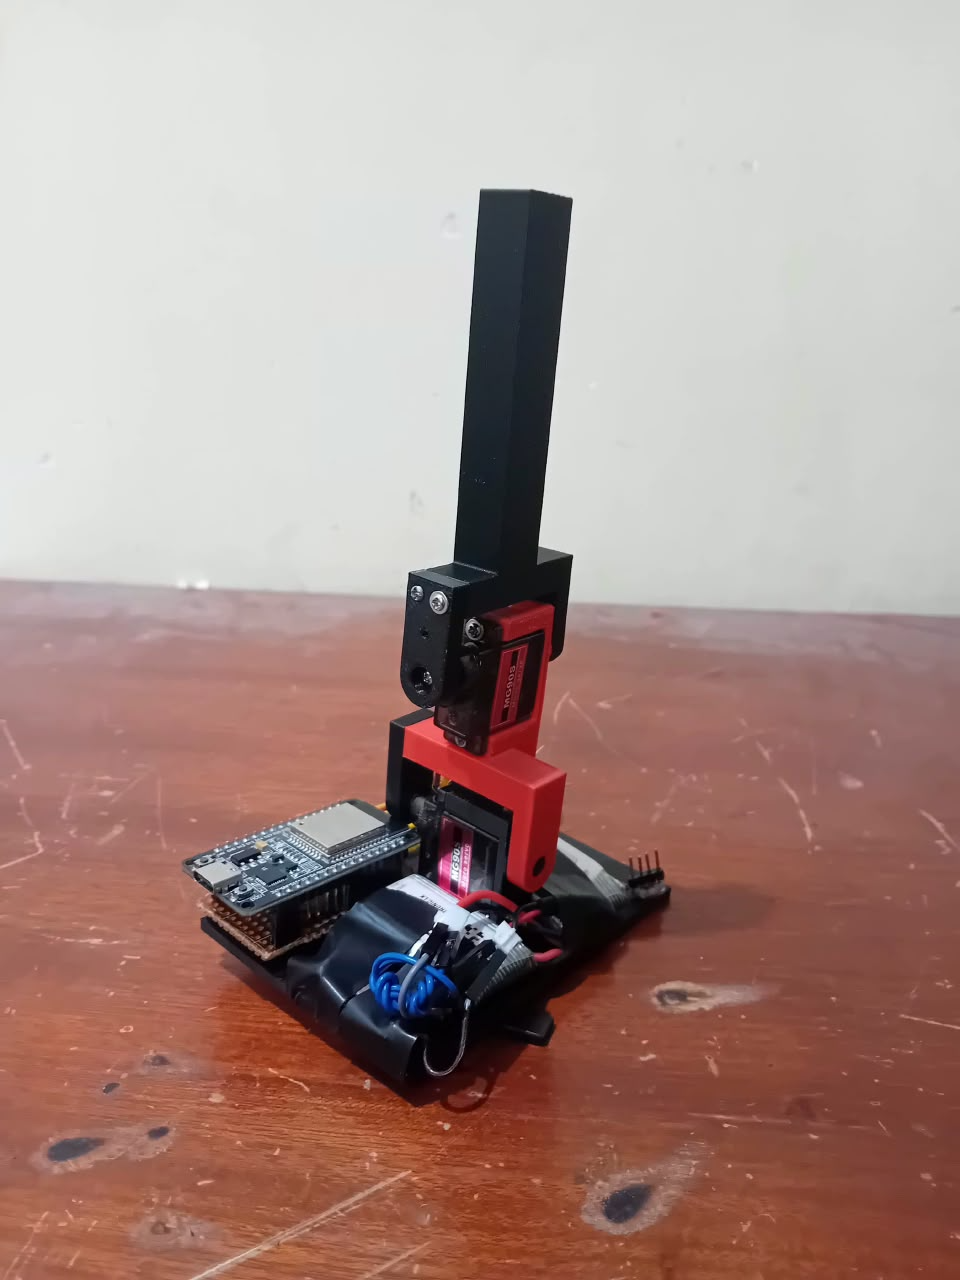
\includegraphics[trim=140bp 110bp 140bp 90bp, clip, height=7.4cm, keepaspectratio]{image.png}\\[0.2em]
    \small \textbf{(b) 3D-Printed Physical \textit{Robo1}}
  \end{minipage}

  \vspace{0.3em}
  \raggedright
  \normalsize
  \textbf{System Specifications \& Training Setup:}
  \begin{itemize}
    \setlength{\itemsep}{0.15em}
    \item \textbf{Kinematics \& Mass:} 2-DOF dynamic self-righting robot ($M = 94.8$\,g, $H = 145$\,mm). Joint 1 (Roll) + Joint 2 (Pitch) actuated by SG90 micro-servos.
    \item \textbf{Embedded Core:} ESP32 dual-core MCU, MPU-6050 6-axis IMU over I2C ($400$\,kHz).
    \item \textbf{Control Policy:} 5-64-64-2 $\tanh$ MLP actor ($4{,}674$ parameters, 18.7\,kB).
    \item \textbf{Observation \& Action:} $\mathbf{o}_t = [\phi_{\text{roll}}, \theta_{\text{pitch}}, a_z, q_1, q_2]$, Action $\Delta q \in [-0.08, +0.08]$\,rad at 50\,Hz.
    \item \textbf{Domain Randomization:} Body mass ($\pm15\%$), damping ($\pm20\%$), motor gain ($\pm15\%$), sensor noise ($\sigma = 0.015$\,rad).
  \end{itemize}
}

% --- Block 5: Experimental Results & Benchmarks ---
\block{\bfseries 5. Experimental Results \& Performance Benchmarks}{
  \small
  \setlength{\tabcolsep}{5.5pt}
  \renewcommand{\arraystretch}{1.18}
  \begin{tabularx}{\linewidth}{p{5.6cm}p{4.2cm}X}
    \toprule
    \rowcolor{TableHeadBg}
    \textbf{Evaluation Domain} & \textbf{Evaluated Target} & \textbf{Measured Metric \& Empirical Findings} \\
    \midrule
    \textbf{Host Numerical Parity} ($n=4{,}609$) & MicroPython Target & Max Abs Error: $\mathbf{1.2 \times 10^{-6}}$ (100\% sign match) \\
    \textbf{Host Numerical Parity} ($n=4{,}609$) & C Header Target & Max Abs Error: $\mathbf{2.9 \times 10^{-6}}$ (100\% sign match) \\
    \midrule
    \textbf{MuJoCo Nominal Righting} & C Header Controller & \textbf{97.2\% Success} (100\% standard falls in 1.15\,s mean) \\
    \textbf{MuJoCo Domain-Rand Physics} & C Header Controller & \textbf{97.2\% Success} (1.38\,s mean get-up time, high robustness) \\
    \midrule
    \textbf{ESP32 Flash Footprint} & Compiled Binary & \textbf{75.1\,kB} (fits standard 4\,MB Flash easily) \\
    \textbf{ESP32 MicroPython RAM} & MicroPython Heap & 119.6\,kB (72\% of free heap; avoids heap thrashing) \\
    \textbf{Hardware I/O Budget (50\,Hz)} & I2C IMU + PWM & \textbf{4.2\,ms} (Only 21\% of 20\,ms real-time deadline) \\
    \textbf{Inference Latency Profile} & MicroPython & $155.2 \pm 7.4$\,ms $\rightarrow$ Compiled C header required for 50\,Hz \\
    \bottomrule
  \end{tabularx}

  \vspace{0.3em}
  \normalsize
  \textbf{Benchmark Findings:}
  \begin{itemize}
    \setlength{\itemsep}{0.15em}
    \item \textbf{Numerical Equivalence:} Single-precision float parity confirmed with max error $<3 \times 10^{-6}$ against PyTorch.
    \item \textbf{Hardware I/O Deadlines:} Peripheral access takes only 4.2\,ms (21\% of 20\,ms budget), proving real-time feasibility.
    \item \textbf{Zero-Heap C Header:} Eliminates interpreted bytecode latency, delivering deterministic 50\,Hz closed-loop control.
  \end{itemize}
}

% --- Block 6: Conclusion & References ---
\block{\bfseries 6. Conclusion \& References}{
  \normalsize
  \textbf{Conclusion:} The \texttt{simtoreal} framework bridges Python RL development and bare-metal microcontroller execution. Evaluations confirm numerical parity and 97.2\% dynamic get-up success in MuJoCo, paving the way for real-world dynamic trials.

  \vspace{0.2em}
  \scriptsize
  \textbf{References:}
  [1] Hwangbo et al., \textit{Sci. Robot.} 2019. \quad
  [2] Rudin et al., \textit{CoRL} 2022. \quad
  [3] Mittal et al., \textit{IEEE RA-L} 2023. \quad
  [4] David et al., \textit{MLSys} 2021. \quad
  [5] Lin et al., \textit{NeurIPS} 2020. \quad
  [6] Eschmann et al., \textit{JMLR} 2024.
}

\end{columns}

\end{document}
